\documentclass[../main.tex]{subfiles}
\graphicspath{{\subfix{../images/}}}
\begin{document}



The so--called peripheral autonomous (vegetative) part of the nervous system\index{nervous system!autonomous!peripheral} is the closest connection
between the semi--autonomous neuronal networks of the small brain of the heart\index{heart!brain} and the emotional brain.
This connection manages the operations of our organs, but totally eludes our will and awareness.
The heart and our emotional brain interact and influence each others.
They build a veritable heart--brain system.\index{nervous system!autonomous}

The \emph{autonomous nervous system}\index{nervous system!autonomous} has a very importance position.
It consists of two strands which originate in the emotional brain and stimulate all organs of the body.
The one strand, called the sympathetic\footnote{The expression ``sympathetic'' has a Latin roots and means ``to be in connection''.
  The nerves of sympathetic nervous system are connected with the spine all along the whole spinal column.} nerve,\index{nerve!sympathetic} 
releases adrenaline and noradrenaline and regulates the fight and flight\index{reaction!fight and flight} reactions.
He increases the heart rate and activates the emotional brain.
The other strand of the autonomous nervous system is the antagonist of the sympathetic nerve and is therefore called the parasympathetic nerve.\index{nerve!parasympathetic}
It releases the neuro transmitter acetylcholine\index{acetylcholine}, which is active in relation with the states of relaxation.
Acetylcholine decreases the heart rate.

The interplay of these two systems can be compared with the \emph{gas pedal} and the \emph{brakes}.
In mammals, these two systems are constantly in equilibrium.
This advantage allows them to adapt extremely fast to changes in their environment.
For instance a rabbit eating herbs in front of his burrow can stop for a moment, put their ears up, listens and sniffles to detect a potential predator.
Is there no sign of danger, it immediately returns to it's meal.
Only mammals have this adaptation.

        \begin{figure}[htb!]
          \centering
          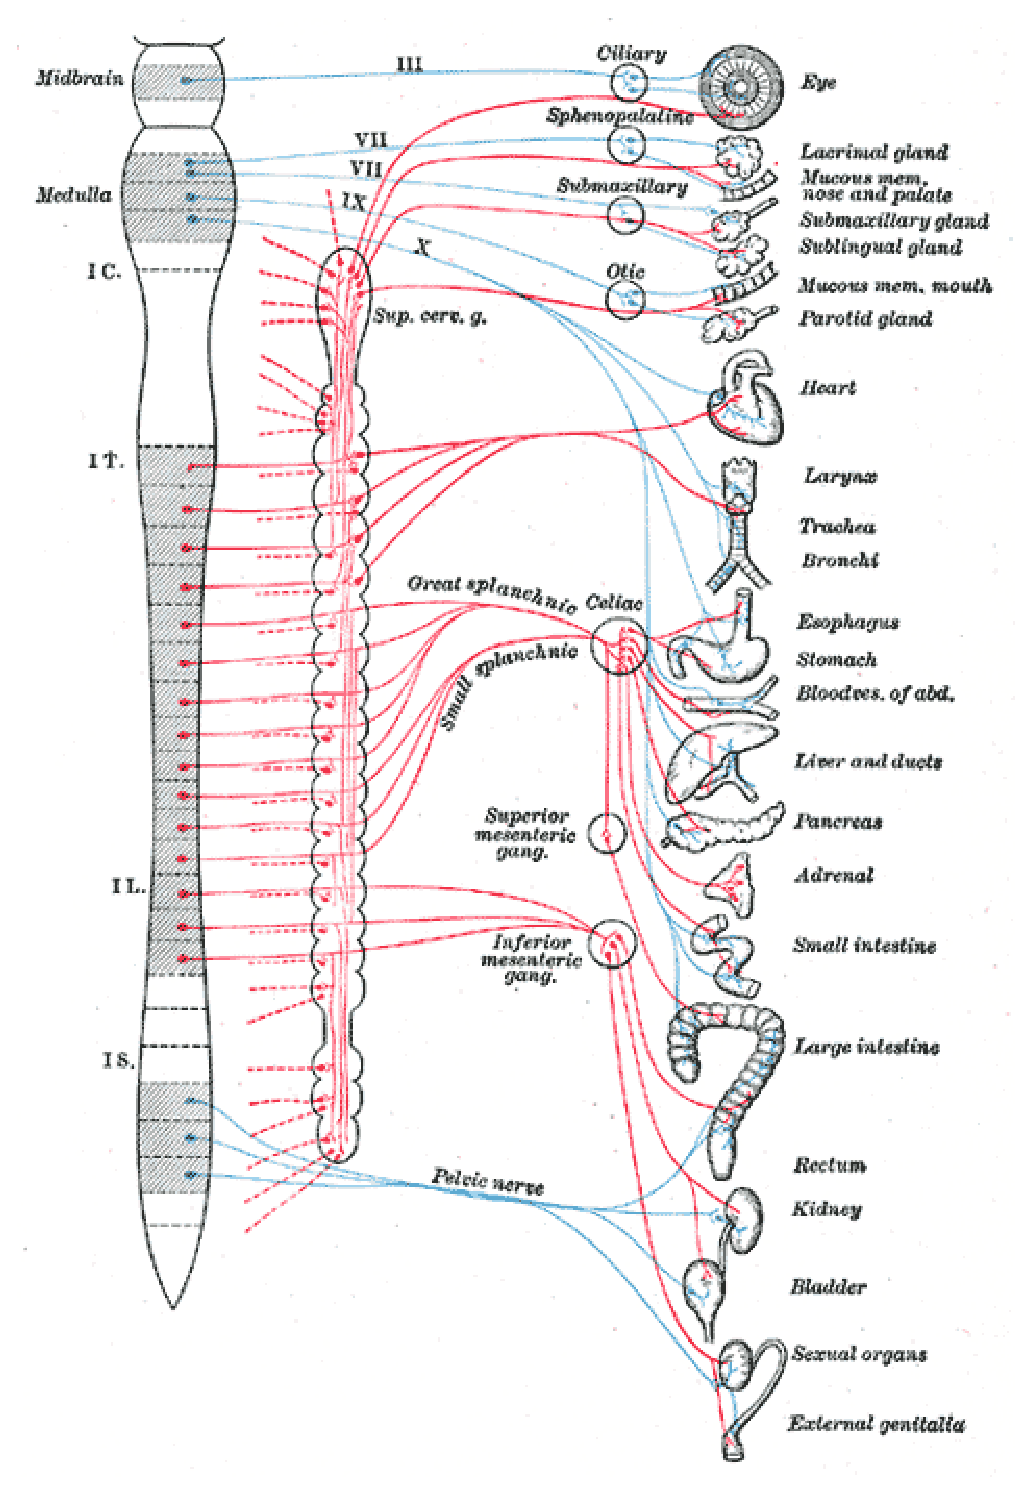
\includegraphics[width=12cm]{AutonomousNS}
          \caption[The autonomous nervous system]{The autonomous nervous system:
            Diagram of efferent sympathetic (red) and parasympathetic (blue) nervous system.~\cite{LeaAnatomy} over~\cite{Bartleby}}\label{pic:AutonomouNS}
        \end{figure}


\end{document}